\chapter{Results}

\begin{figure}[ht]
    \centering
	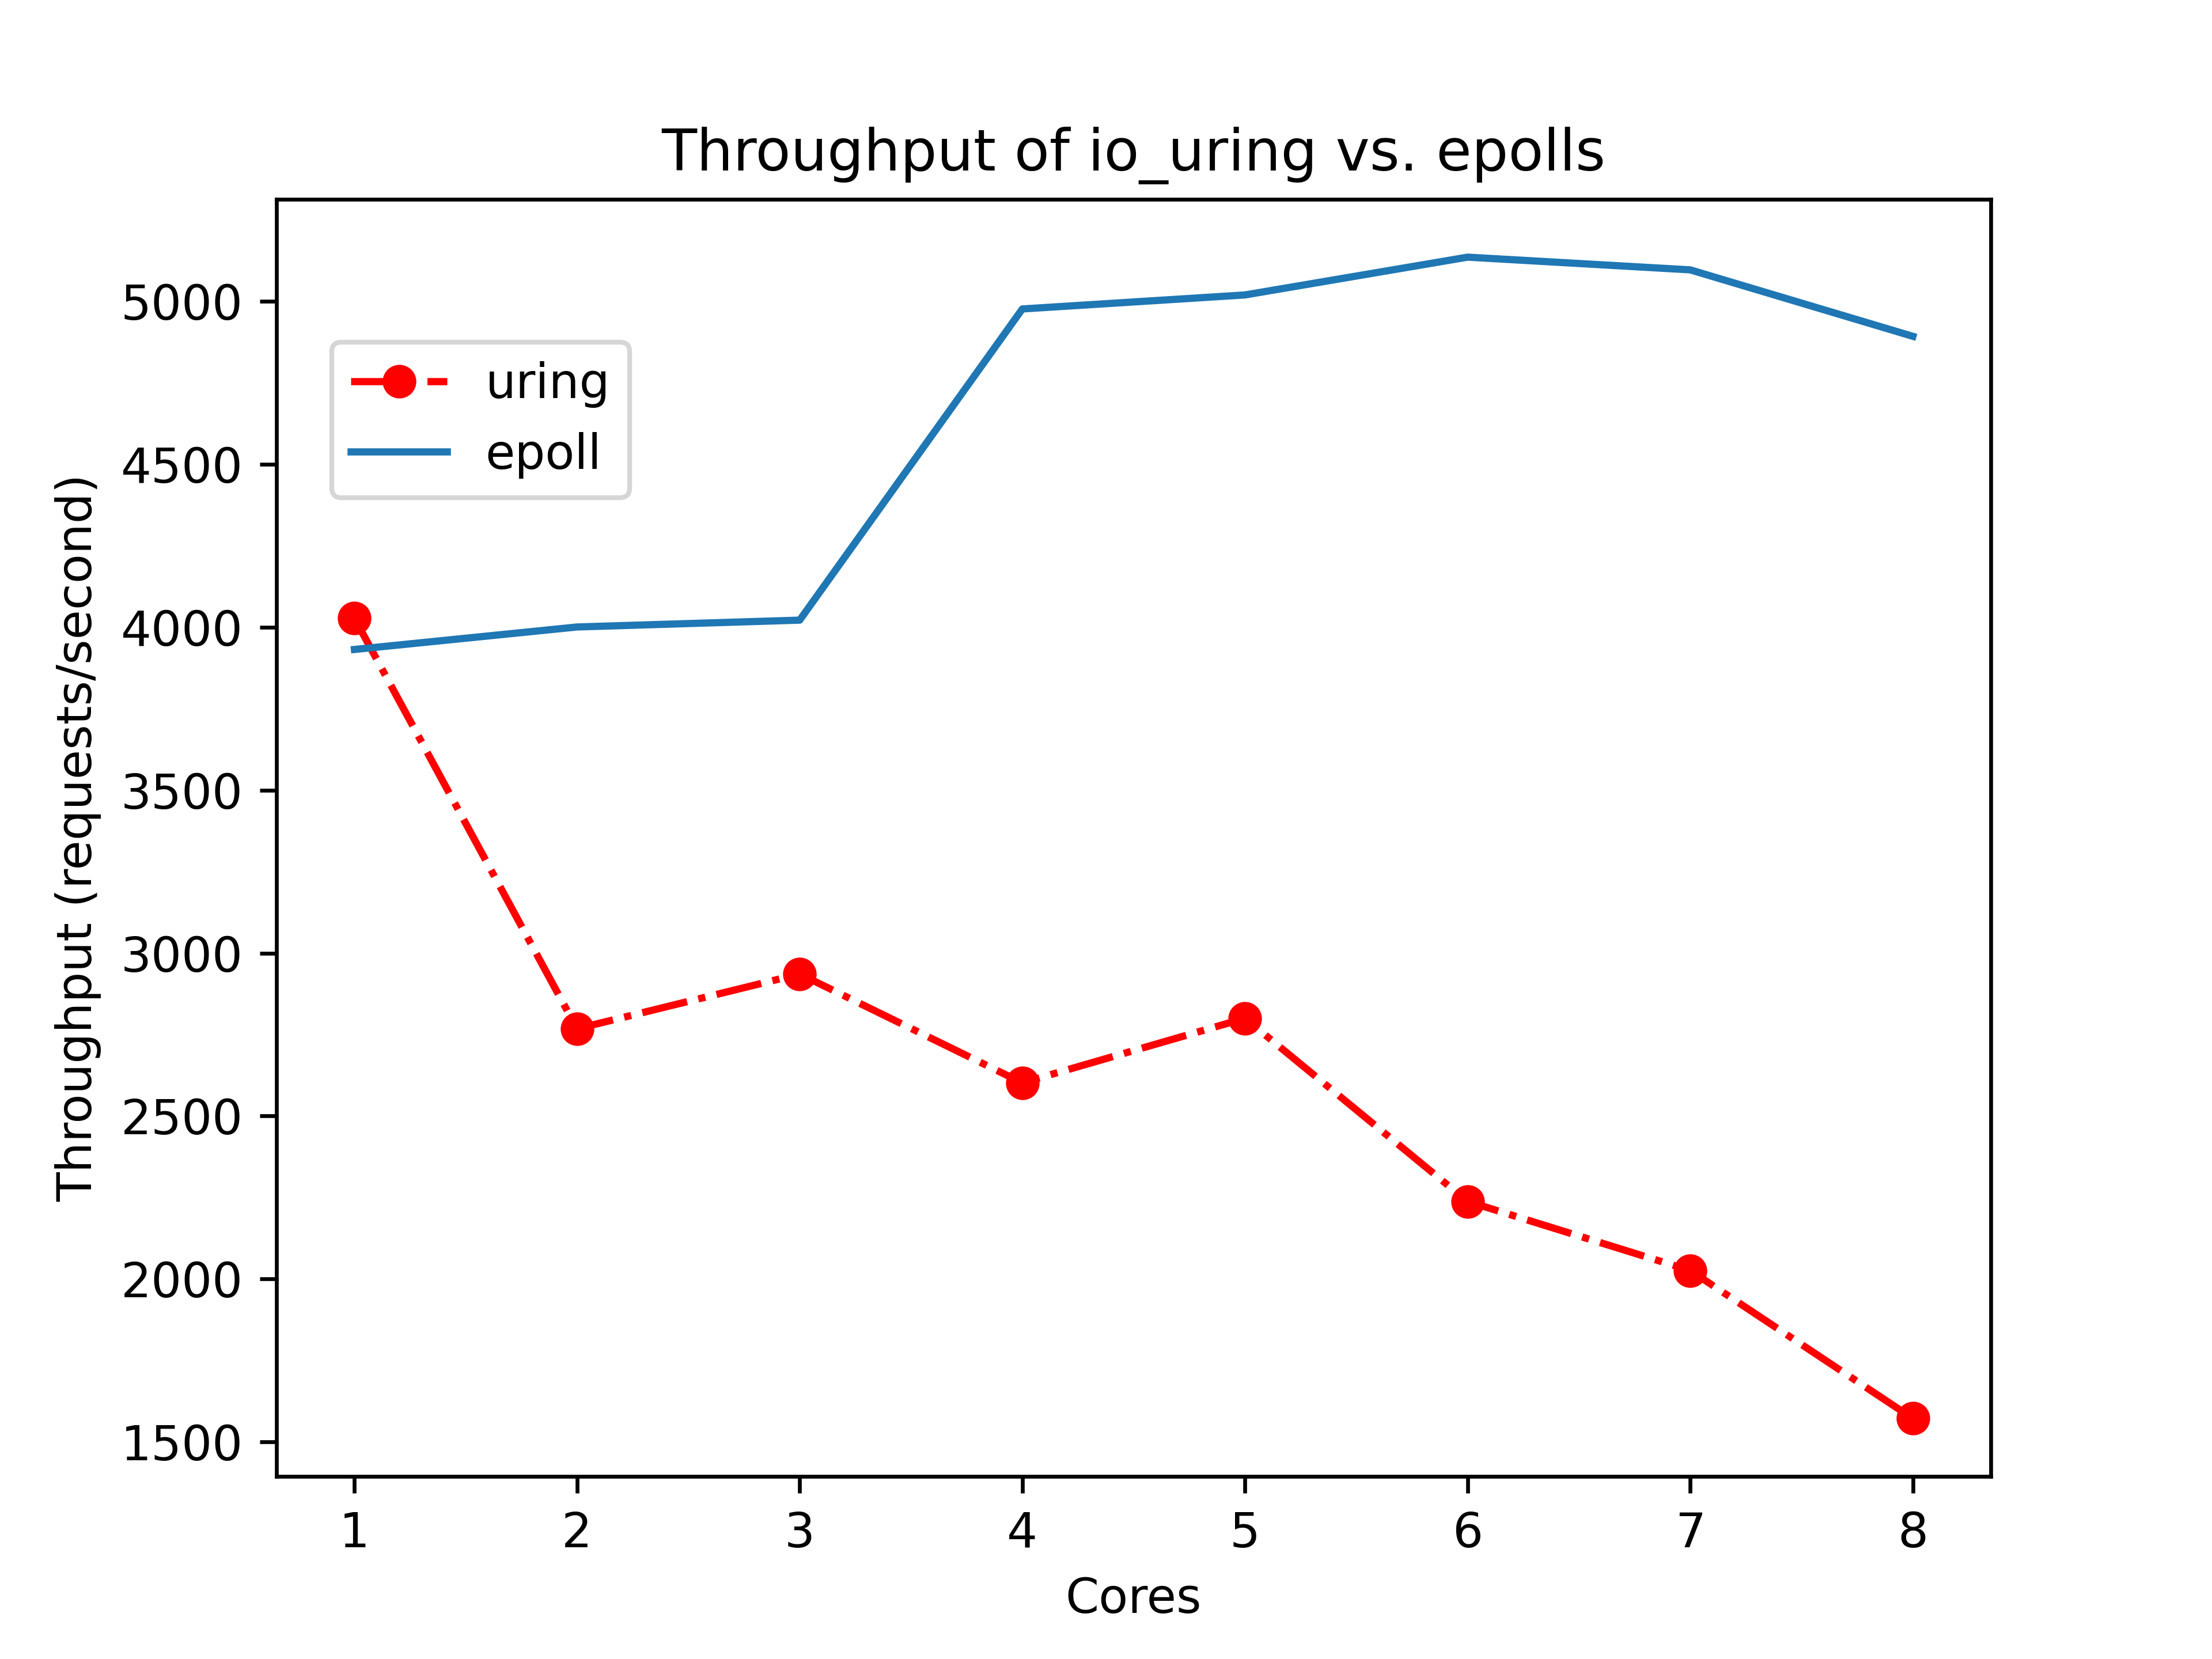
\includegraphics[width=0.85\textwidth]{figures/graphics/throughput.png}
	\caption[Web Server Throughput]{
		Graph comparing the throughput of the \texttt{io\_uring URingManager} web server
		and the \texttt{epoll EventManager} web server. Benchmarked by sending
		10,000 requests and 50 concurrent connections
	}
	\label{fig:throughput}
\end{figure}

For this section, we will refer to the \texttt{io\_uring} case interchangeably as the \texttt{URingManager} case, and likewise for epoll being interchangeable with \texttt{EventManager}.

In the single-Capability case, with 50 concurrent connections, and \texttt{URingManager} at 4028 kilobytes per second vs. \texttt{EventManager} at 3923 kilobytes per second, \texttt{io\_uring} has a very negligible lead in throughput over epoll. However, \texttt{io\_uring} performance worsens as the Capability count increases. As for \texttt{EventManager}, throughput increases slightly as Capability count increases up until it plateaus at around 6 Capabilities. These observations
regarding throughput can be seen from Figure \ref{fig:throughput}. 

\begin{figure}[ht]
    \centering
	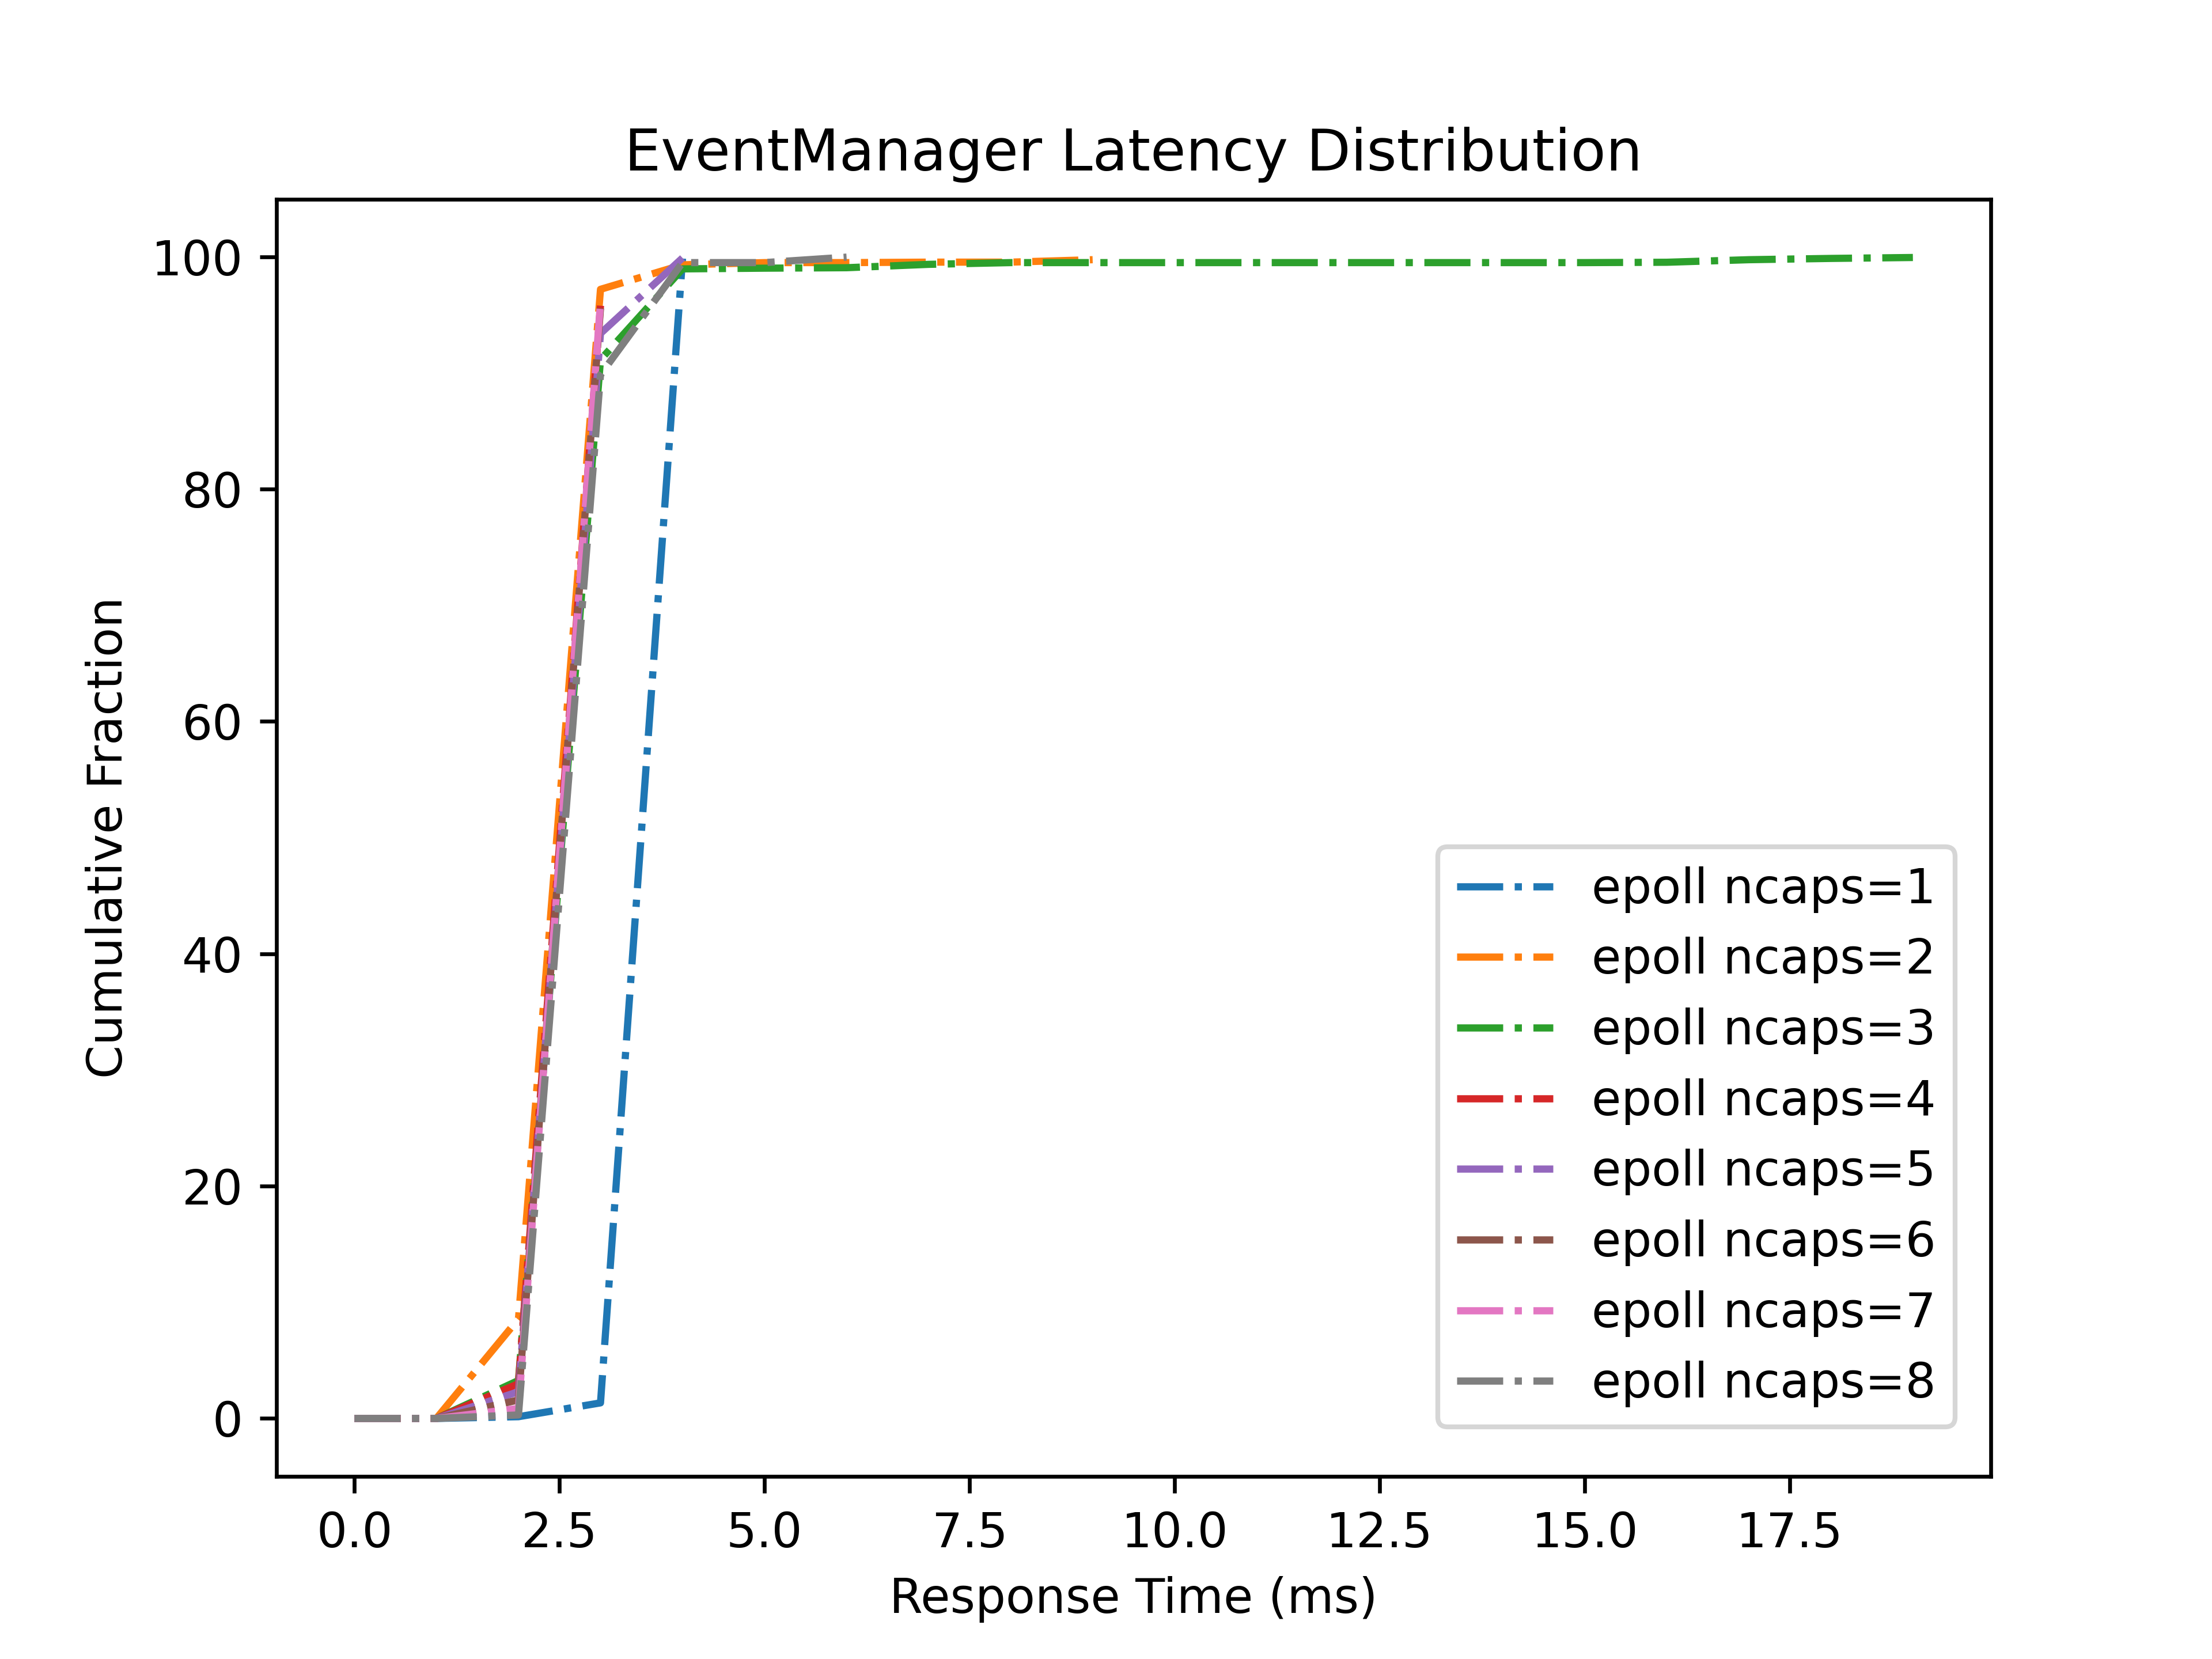
\includegraphics[width=0.85\textwidth]{figures/graphics/epoll_latency.png}
	\caption[\texttt{epoll EventManager} Web Server Latency]{
		Cumulative Distribution of latencies of the \texttt{epoll EventManager} web server
		program over 10,000 requests and 50 concurrent connections
	}
	\label{fig:epoll_latency}
\end{figure}

\begin{figure}[ht]
    \centering
	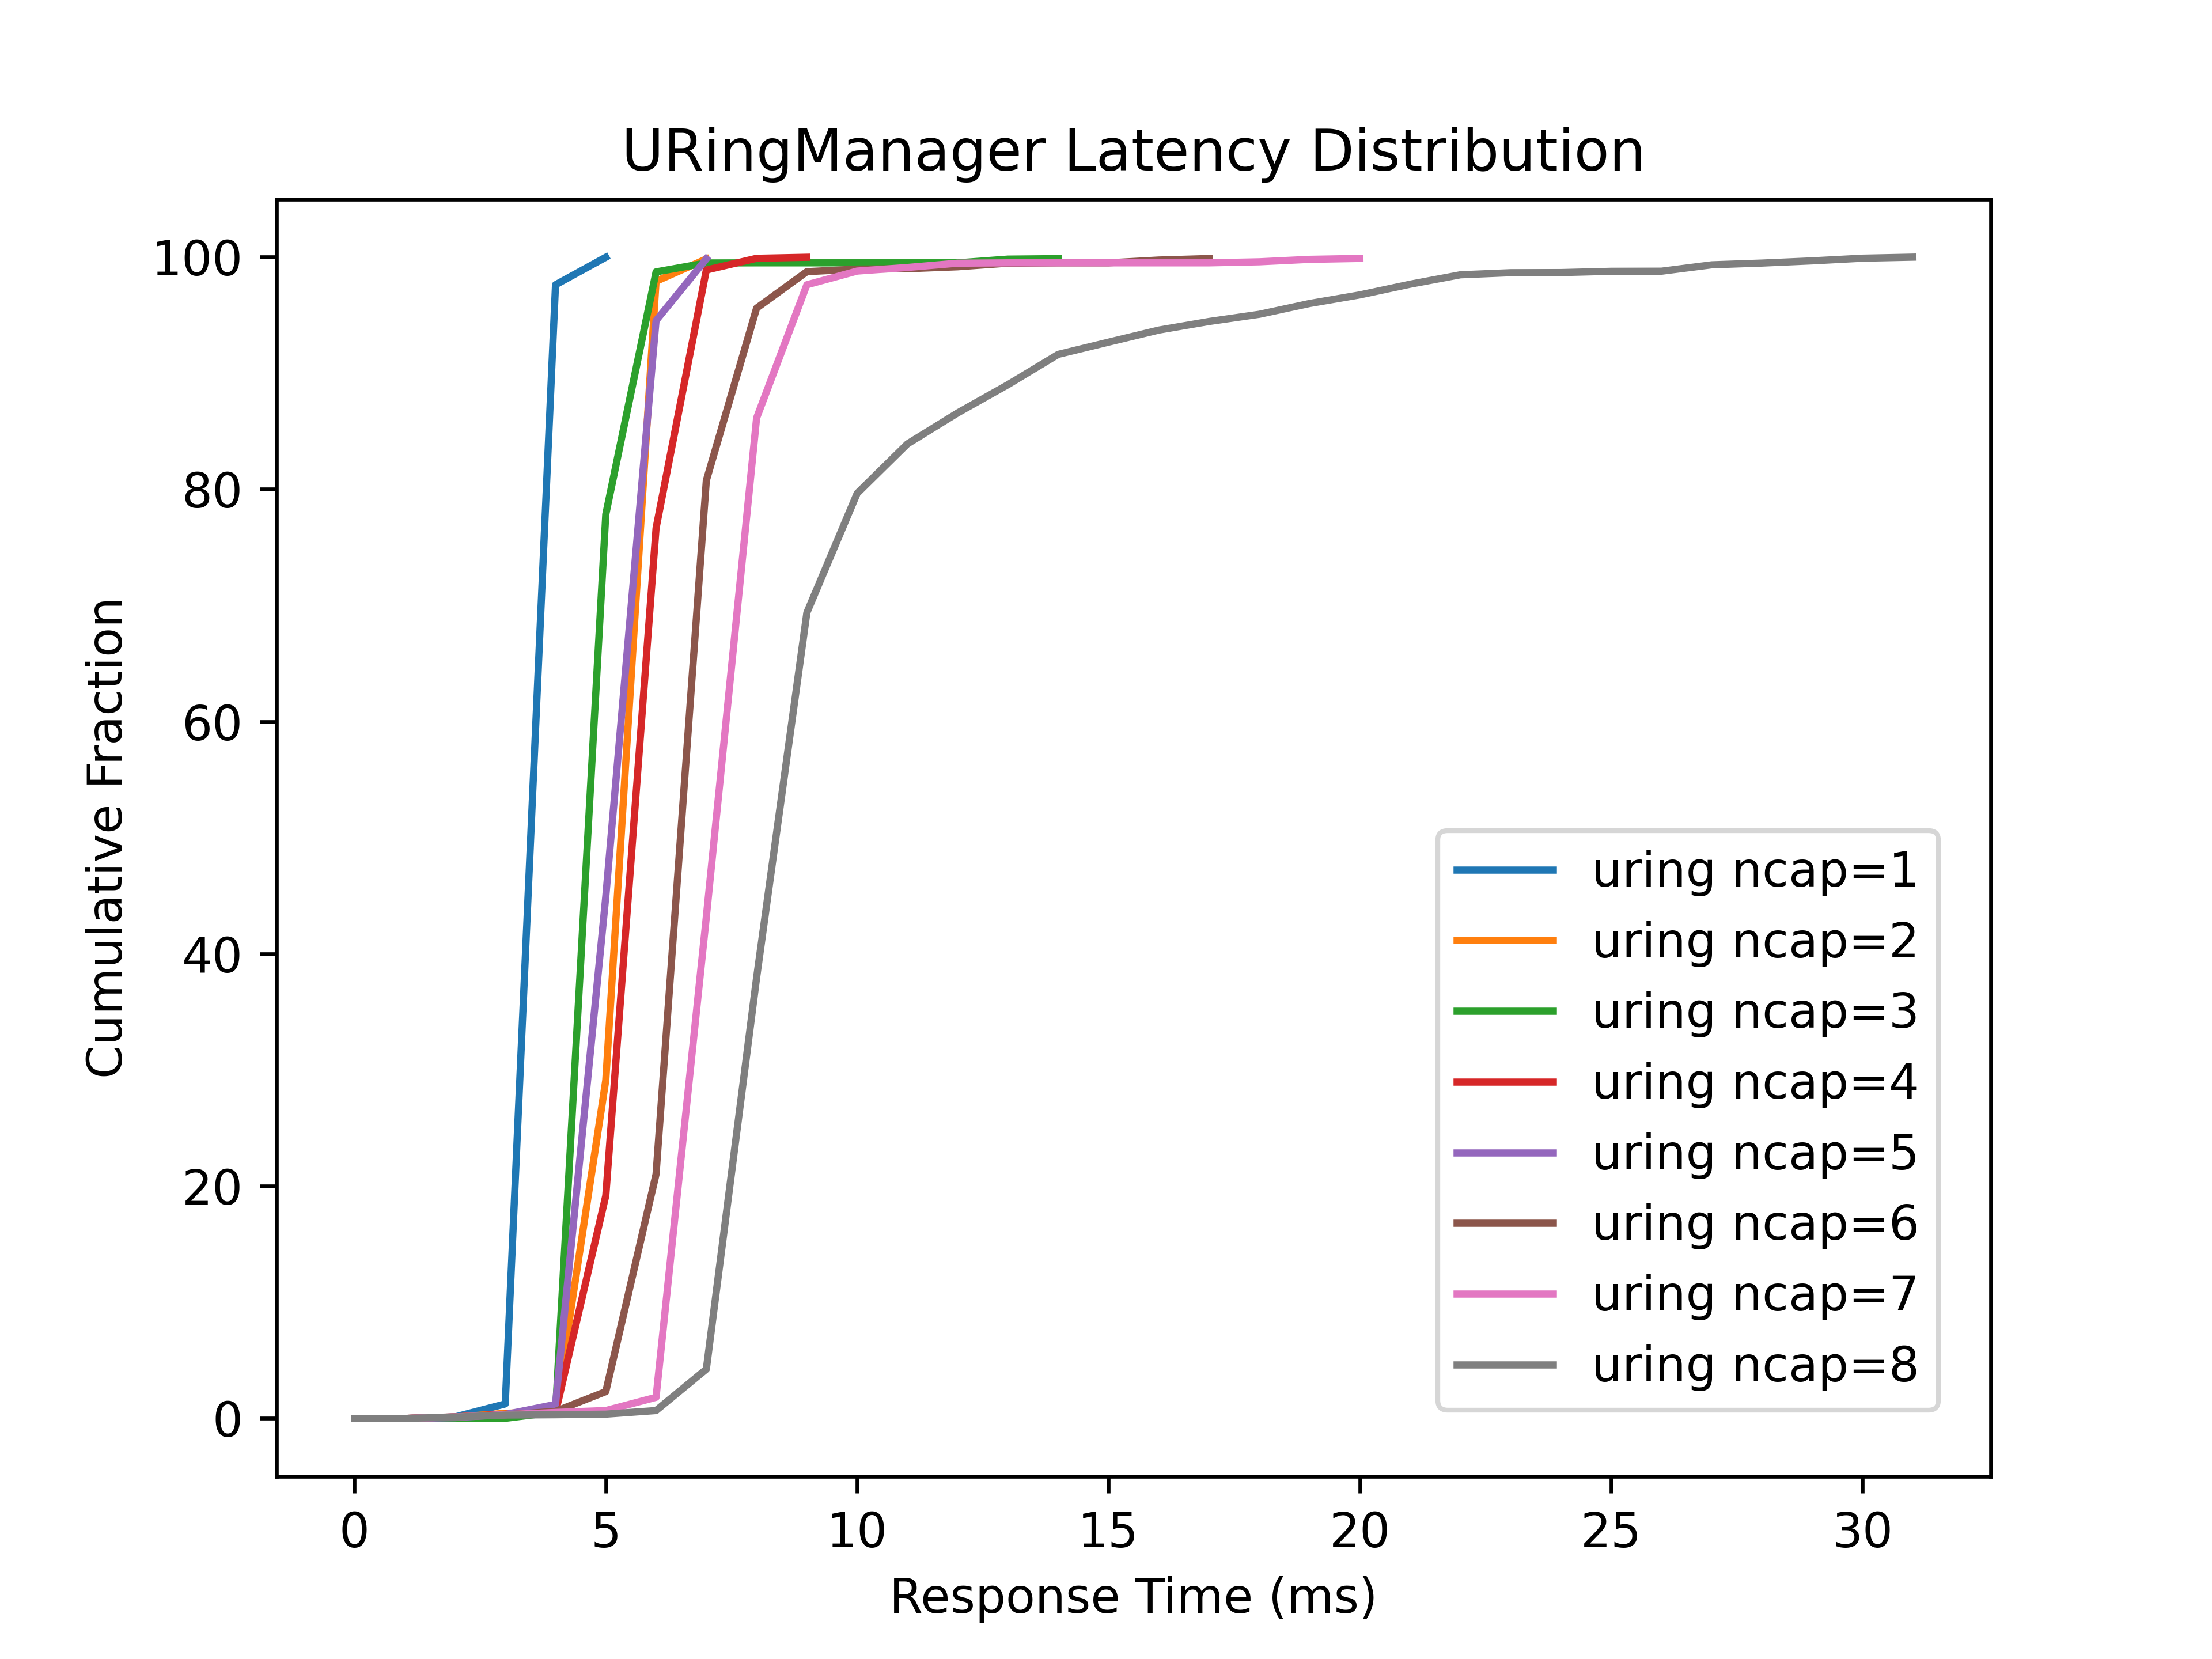
\includegraphics[width=0.85\textwidth]{figures/graphics/uring_latency.png}
	\caption[\texttt{io\_uring URingManager} Web Server Latency]{
		Cumulative Distribution of latencies of the \texttt{io\_uring URingManager} web server
		program over 10,000 requests and 50 concurrent connections
	}
	\label{fig:uring_latency}
\end{figure} 


As for tail latency, the single core \texttt{io\_uring} case is comparable to
\texttt{epoll} as shown in the Cumulative Fraction graphs.
Like with throughput, tail latency is worse as the number of URingManager capabilities increase;
compare Figure \ref{fig:epoll_latency} and \ref{fig:uring_latency}.